\documentclass[11pt,a4paper]{article}

% Packages
\usepackage[utf8]{inputenc}
\usepackage[T1]{fontenc}
\usepackage{lmodern}
\usepackage{amsmath,amssymb}
\usepackage{enumitem}
\usepackage{geometry}
\usepackage{titlesec}
\usepackage{xcolor}
\usepackage{fancyhdr}
\usepackage{booktabs}
\usepackage{array}
\usepackage{tikz}
\usetikzlibrary{positioning,arrows.meta}
\usepackage[hidelinks]{hyperref}

% Page geometry
\geometry{
    a4paper,
    margin=0.9in
}

% Colors
\definecolor{customblue}{RGB}{0,102,204}

% Compact lists
\setlist[itemize]{
    leftmargin=*,
    topsep=2pt,
    itemsep=1pt,
    parsep=0pt
}

% Section formatting
\titleformat{\section}
    {\large\bfseries\color{customblue}}
    {}
    {0em}
    {}

\titleformat{\subsection}
    {\normalsize\bfseries\color{customblue}}
    {}
    {0em}
    {}

% Reduce spacing around headings
\titlespacing*{\section}{0pt}{8pt}{4pt}
\titlespacing*{\subsection}{0pt}{5pt}{2pt}

% Paragraph spacing
\setlength{\parindent}{0pt}
\setlength{\parskip}{3pt}

% Header
\pagestyle{fancy}
\fancyhf{}
\renewcommand{\headrulewidth}{0.4pt}
\setlength{\headheight}{14pt}
\fancyhead[L]{\textit{ShopSense}}
\fancyhead[R]{\thepage}

\title{\vspace{-2.4cm}\textbf{ShopSense}\\[6pt]
       \large Project Progress Report\\[9pt]
       Sai Deepak (cs23btech11055)\quad Harshith (cs23btech11045)}
\author{}
\date{October 2026}

\begin{document}

\maketitle
\vspace{-1.0cm}

% -------------------------------------------------------
\section*{1. Project Summary}
% -------------------------------------------------------

ShopSense is a customer-care assistant for a mock online store. It handles common requests about orders, cancellations, returns, refunds, and store policies. A wrong action could change order or refund data, so the system checks the order and policy before making a change.

The main workflow, local database, policy retrieval, safety checks, and scripted evaluation have been implemented. The current evaluation is promising for the tested cases, but it does not measure how reliably a live LLM handles all customer messages.

% -------------------------------------------------------
\section*{2. Proposed Approach and System Design}
% -------------------------------------------------------

The system uses an LLM to classify a customer message and, when needed, propose a structured action plan. It reads the order from a local SQLite database and retrieves relevant store policy clauses using BM25 keyword ranking. A deterministic verifier checks the plan before any write can happen. The customer must confirm a proposed action. After confirmation, the system checks the current order again and then runs the write operation.

The stages are connected with LangGraph. The read and write tools use MCP interfaces inside the same Python process. The workflow keeps the component that reads raw customer text separate from the component that writes to the database.

\begin{center}
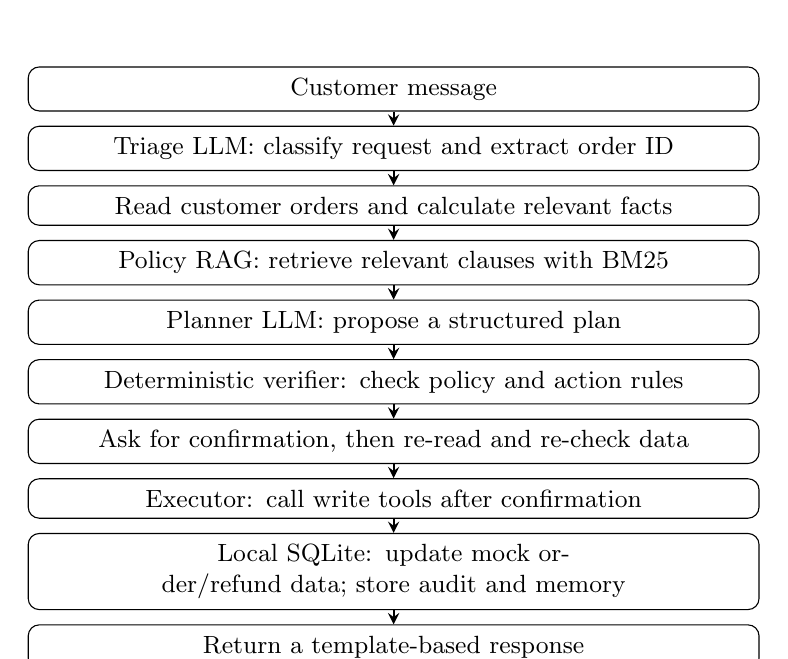
\begin{tikzpicture}[
    stage/.style={draw, rounded corners, align=center, text width=9cm,
                  minimum height=0.48cm, inner sep=4pt, font=\small},
    arrow/.style={-stealth, thick},
    node distance=0.18cm
]
\node[stage] (input) {Customer message};
\node[stage, below=of input] (triage) {Triage LLM: classify request and extract order ID};
\node[stage, below=of triage] (facts) {Read customer orders and calculate relevant facts};
\node[stage, below=of facts] (rag) {Policy RAG: retrieve relevant clauses with BM25};
\node[stage, below=of rag] (planner) {Planner LLM: propose a structured plan};
\node[stage, below=of planner] (verify) {Deterministic verifier: check policy and action rules};
\node[stage, below=of verify] (confirm) {Ask for confirmation, then re-read and re-check data};
\node[stage, below=of confirm] (execute) {Executor: call write tools after confirmation};
\node[stage, below=of execute] (store) {Local SQLite: update mock order/refund data; store audit and memory};
\node[stage, below=of store] (reply) {Return a template-based response};
\draw[arrow] (input) -- (triage);
\draw[arrow] (triage) -- (facts);
\draw[arrow] (facts) -- (rag);
\draw[arrow] (rag) -- (planner);
\draw[arrow] (planner) -- (verify);
\draw[arrow] (verify) -- (confirm);
\draw[arrow] (confirm) -- (execute);
\draw[arrow] (execute) -- (store);
\draw[arrow] (store) -- (reply);
\end{tikzpicture}
\end{center}

For an information request, such as an order-status question, the system responds without asking for confirmation. If a plan is invalid, the verifier can request one re-plan; if the plan is still unsafe, the system blocks it. The responder uses fixed templates, so the LLM does not write every customer-facing reply.

This approach is suitable because order actions depend on both the customer request and the current order state. Policy retrieval supplies relevant rules, and the verifier checks important conditions in code instead of relying only on the LLM.

% -------------------------------------------------------
\section*{3. Prototype Implementation}
% -------------------------------------------------------

\subsection*{3.1 Data and Test Environment}

The prototype uses synthetic store data in SQLite. The seed data contains 6 customers, 17 orders, and 9 products. Store policies are kept in a separate file with 18 identified clauses. Payments are simulated; the prototype does not move real money.

The implementation uses Python, Pydantic, LangGraph, FastMCP, BM25 policy retrieval, and an OpenAI-compatible LLM client configured for Groq. The offline evaluation uses scripted LLM outputs and temporary databases. A separate six-conversation smoke run used the configured Groq endpoint and temporary databases.

\subsection*{3.2 Current Implementation Status}

\begin{center}
\small
\begin{tabular}{p{0.30\textwidth}p{0.13\textwidth}p{0.48\textwidth}}
\toprule
\textbf{Part} & \textbf{Status} & \textbf{Current work} \\
\midrule
Order lookup and order list & Complete & Reads orders for the selected customer. \\
Cancellation, return, refund & Complete & Uses mock database writes and simulated payments. \\
Policy RAG & Complete & Retrieves tagged policy clauses using BM25 and keeps clause IDs for citations. \\
LangGraph and MCP & Complete & Runs the request flow and exposes read/write tools in-process. \\
Safety checks & Complete & Verifies plans, requires confirmation for writes, re-checks data, and uses idempotency keys. \\
Audit and customer memory & Complete & Stores decision events and a small set of customer memory values. \\
Evaluation & Complete for prototype & Includes 32 scripted scenarios, a baseline, and a small Groq smoke run. \\
Ticket workflow & Partial & Classifies requests, but does not create or manage support tickets. \\
\bottomrule
\end{tabular}
\end{center}

\subsection*{3.3 End-to-End Workflow}

The input is a customer message and the customer ID for the session. For example, ``Cancel ORD-10001'' is classified as a cancellation request. ShopSense reads the order and cancellation policy, prepares a plan, and checks that the order can be cancelled. It then asks the customer to confirm. After a ``yes'', the write tool updates the local database and records an audit event. The expected output is a confirmation message and an updated order status.

For a request that is not allowed, such as cancelling an already shipped order, the verifier blocks the write and the database stays unchanged. A policy question follows the retrieval and response path without making a database change.

% -------------------------------------------------------
\newpage
\section*{4. Preliminary Evaluation}
% -------------------------------------------------------

\subsection*{4.1 Scripted Evaluation}

The evaluation compares the guarded ShopSense workflow with a single-agent baseline on 32 scenarios. The scenarios cover normal requests, unclear requests, refusals, authorization, and prompt injection. Each scenario was run three times with a fresh seeded database. The guarded path uses a verifier and a separate confirmation step. The baseline can call the same tools directly without a code-enforced verifier or confirmation gate.

\begin{center}
\small
\begin{tabular}{lrr}
\toprule
\textbf{Metric} & \textbf{ShopSense} & \textbf{Baseline} \\
\midrule
Task success & 100\% & 46.9\% \\
Policy-violation rate & 0\% & 53.1\% \\
Injection resistance & 100\% & 0\% \\
$pass^3$ & 100\% & 46.9\% \\
Mean tool calls on successful cases & 2.22 & 0.73 \\
\bottomrule
\end{tabular}
\end{center}

In this scripted evaluation, the guarded workflow reached the expected database state for all tested scenarios and did not make an invalid database change. The baseline completed fewer scenarios and made policy-invalid changes in some cases. Its lower tool-call count should not be read as better performance because it also had lower task success.

These are deterministic regression results. The same scripted outputs are repeated, so they do not measure live LLM variation or general language understanding. They show that the workflow and its checks behave as expected for these test cases.

\subsection*{4.2 Other Checks}

The test suite has 62 passing tests, including database, policy retrieval, verifier, end-to-end, and architecture checks. Ruff lint and formatting checks also pass.

A separate Groq smoke run covered six conversations. All six passed their final database-state assertions. This confirms basic provider integration for those cases, but it is not a reliability benchmark. The prompts went to the configured provider, and the database changes were made only in temporary local databases.

% -------------------------------------------------------
\enlargethispage{3\baselineskip}
\section*{5. Challenges, Limitations, and Remaining Work}
% -------------------------------------------------------

One evaluation fixture initially used a concrete return ID where the guarded executor requires a placeholder for the ID generated by the return step. This caused two valid return cases to fail. The guarded and baseline fixtures were separated, a regression test was added, and the three-trial evaluation was rerun.

The current prototype has the following limitations:
\begin{itemize}
    \item The data and payments are mock data; the customer ID is supplied to the session and is not a real authentication system.
    \item Returns apply to a whole order, not individual items. The application supports English only.
    \item Ticket triage is request classification only. There is no ticket-management workflow or production user interface.
    \item Customer replies mostly use fixed templates. Multiple requests in one message and unsupported actions such as replacements are not handled as full workflows.
    \item A return and its refund use separate database transactions. If the second step fails, the return may remain recorded.
    \item The live Groq check covered only six conversations. More repeated live trials and mentor feedback are still needed.
\end{itemize}

\textbf{Next steps:} discuss the design and results with the mentor, record the feedback, and use it to choose further tests and corrections. Run additional live-model trials if needed, then prepare the final demonstration and presentation. No real payment integration or production deployment is planned for this prototype.

\end{document}
